\documentclass{article}
\usepackage{cmap}
\usepackage[utf8]{inputenc}
\usepackage[english,ukrainian]{babel}
\usepackage{graphicx}
\usepackage{geometry}
\usepackage{listings}
\usepackage{float}
\usepackage{amsmath}
\usepackage{subfig}
\usepackage{xcolor}
\geometry{
	a4paper,
	left=20mm,
	right=20mm,
	top=15mm,
	bottom=15mm,
}
\lstset{
	tabsize=4,
	keepspaces,
	showstringspaces=false,
	escapeinside={(*@}{@*)},
	breaklines,
}
\graphicspath{ {./pictures} }
\setlength{\parindent}{4em}

\newcommand\subject{Архітектура комп'ютера}
\newcommand\lecturer{доцент кафедри ПЗ\\Крук О.Г.}
\newcommand\teacher{доцент кафедри ПЗ\\Крук О.Г.}
\newcommand\mygroup{ПЗ-22}
\newcommand\lab{9}
\newcommand\theme{Складення та відлагодження циклічної програми мовою асемблера процесорів Cortex- M3/M4}
\newcommand\purpose{Ознайомитись на приладі циклічної програми з основними командами асемблера процесорів Cortex- M3/M4; розвинути навики складання програми з вкладеними циклами; відтранслювати і виконати покроково в режимі відлагодження програму, складену відповідно до свого варіанту; перевірити виконання тесту}

\begin{document}
	\begin{normalsize}
		\begin{titlepage}
			\thispagestyle{empty}
			\begin{center}
				\textbf{МІНІСТЕРСТВО ОСВІТИ І НАУКИ УКРАЇНИ\\
					НАЦІОНАЛЬНИЙ УНІВЕРСИТЕТ "ЛЬВІВСЬКА ПОЛІТЕХНІКА"}
			\end{center}
			\begin{flushright}
				\textbf{ІКНІ}\\
				Кафедра \textbf{ПЗ}
			\end{flushright}
			\vspace{200pt}
			\begin{center}
				\textbf{ЗВІТ}\\
				\vspace{10pt}
				до лабораторної роботи № \lab\\
				\textbf{на тему}: “\textit{\theme}”\\
				\textbf{з дисципліни}: “\subject”
			\end{center}
			\vspace{112pt}
			\begin{flushright}
				
				\textbf{Лектор}:\\
				\lecturer\\
				\vspace{28pt}
				\textbf{Виконав}:\\
				
				студент групи \mygroup\\
				Коваленко Д.М.\\
				\vspace{28pt}
				\textbf{Прийняв}:\\
				
				\teacher\\
				
				\vspace{28pt}
				«\rule{1cm}{0.15mm}» \rule{1.5cm}{0.15mm} 2022 р.\\
				$\sum$ = \rule{1cm}{0.15mm}……………\\
				
			\end{flushright}
			\vspace{\fill}
			\begin{center}
				\textbf{Львів — 2022}
			\end{center}
		\end{titlepage}
		
		\begin{description}
			\item[Тема.] \theme.
			\item[Мета.] \purpose.
		\end{description}
		
		\section*{Індивідуальне завдання}
		\begin{figure}[H]
			\centering
			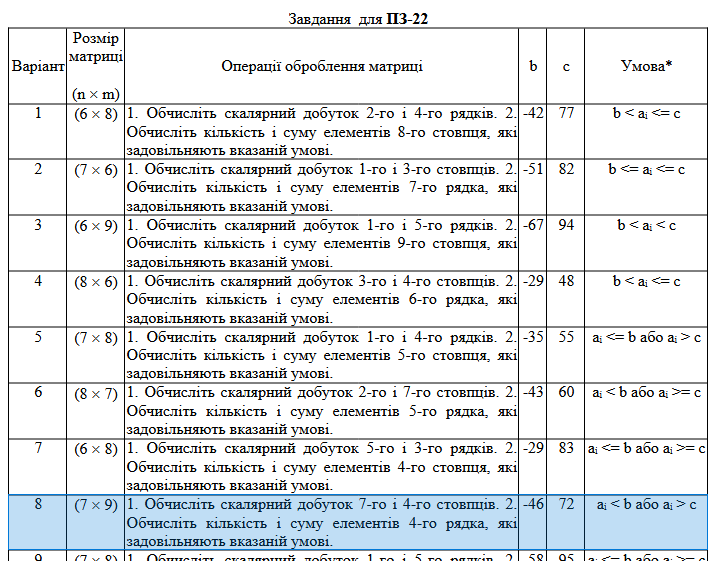
\includegraphics[scale=0.7]{v}
		\end{figure}
		
		\section*{Хід роботи}
		\subsection*{Код програми}
		\begin{lstlisting}
	AREA MyCode, CODE, ReadOnly
ENTRY
EXPORT MyProg
MyProg
TRANSPOSE
LDR r0, = arr
LDR r1, = res
LDR r2, = 7		; rows
LDR r3, = 9		; cols
LDR r7, = 4		; DCD size
LDR r4, = 0		; 0..cols
OUTER
LDR r5, = 0		; 0..rows

INNER
LDR r0, = arr
LDR r1, = res

MUL r6, r5, r3
ADD r6, r4
MUL r6, r6, r7
ADD r0, r6

MUL r6, r4, r2
ADD r6, r5
MUL r6, r6, r7
ADD r1, r6	

LDR r6, [r0]
STR r6, [r1]

ADD r5, #1	
CMP r5, r2
BLO INNER

ADD r4, #1	
CMP r4, r3
BLO OUTER

SCALAR
LDR r0, = arr + 12	; 4 col
LDR r1, = arr + 24	; 7 col
LDR r4, = 7		; rows
LDR r5, = 0		; 0..rows
LDR r6, = 0		; scalar
LDR r7, = scalar

LOOP
LDR r2, [r0]
LDR r3, [r1]
MUL r2, r2, r3
ADD r6, r2
ADD r0, #36
ADD r1, #36
ADD r5, #1
CMP r5, r4
BLO LOOP
STR r6, [r7]

LDR r0, = arr + 108	; 4 row
LDR r3, = 0		; 0..cols
LDR r4, = 0		; sum
LDR r5, = 0		; count
LDR r6, = sum
LDR r7, = count
COUNT_AND_SUM
LDR r1, [r0]
ADD r0, #4

CMP r3, #9
BGE DONE
ADD r3, #1
CMP r1, #-46
BLT DO
CMP r1, #72
BGT DO
B COUNT_AND_SUM

DO
ADD r4, r1
ADD r5, #1
B COUNT_AND_SUM

DONE
STR r4, [r6]
STR r5, [r7]

STOP 		B STOP

ALIGN
AREA InputData, Data, ReadOnly
EXPORT arr
arr		DCD  10, 64,-94, 77, 99, 18, 52,-11, 96
DCD -23,-77,-45, 65, 77, 66,-24, 69,-30
DCD -81,-78,-82,-39,-90,-78, 24, 95,-92
DCD -18,-64,-74,-28,-16,-40, 91, 42,-35
DCD  56,-19, 86, 34,-83,-99,-31,-51, 79
DCD -70,-58, 13, 98, 90, 46,-77, 37, 68
DCD  97, 85,-10, 57, 88, 99,-26,-51,-39

AREA OutputData, Data, ReadWrite
EXPORT res
EXPORT scalar
EXPORT sum
EXPORT count

res 	SPACE 7 * 9 * 2
scalar	SPACE 4
sum		SPACE 4
count	SPACE 4
END
		\end{lstlisting}
		
\section*{Транспонування}
\begin{figure}[H]
	\centering
	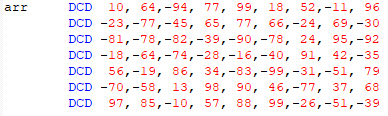
\includegraphics[scale=0.7]{2}
	\caption{Вигляд масиву}
\end{figure}
		
\begin{figure}[H]
	\centering
	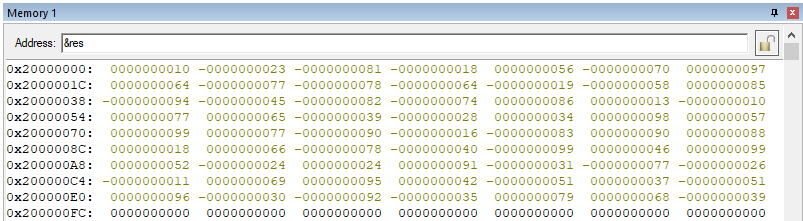
\includegraphics[scale=0.6]{1}
	\caption{Результат транспонування}
\end{figure}

\section*{Скалярний добуток}
Стовпець 4: $a=[77, 65, -39, -28, 34, 98, 57]$\\
Стовпець 7: $b=[52, -24,24,91,-31,-77,-26]$

\noindent Скалярний добуток: 
\begin{gather}
	\sum_{i=0}^{7}a_ib_i=77\cdot52+65\cdot(-24)+(-39)\cdot24+(-28)\cdot91+34\cdot(-31)+98\cdot(-77)+57\cdot(-26)=-11122\nonumber
\end{gather}

\begin{figure}[H]
	\centering
	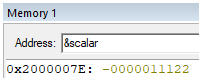
\includegraphics[scale=0.7]{3}
	\caption{Результат обчислення скалярного добутку}
\end{figure}

\section*{Кількість та сума елементів за заданою умовою}
Умова: $a_i<-46$, $a_i>72$\\
Рядок 4: $[-18, -64, -74, -28, -16, -40, 91, 42, -35]$\\
Кількість: 3\\
Сума: $-64-74+91=-47$
\begin{figure}[H]
	\centering
	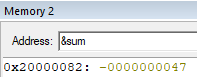
\includegraphics[scale=0.7]{4}
	\caption{Результат обчислення суми елементів за заданою умовою}
\end{figure}

\begin{figure}[H]
	\centering
	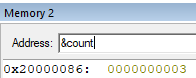
\includegraphics[scale=0.7]{5}
	\caption{Результат обчислення кількості елементів за заданою умовою}
\end{figure}
			
		\section*{Висновки}
		Під час виконання лабораторної роботи я ознайомивсь на приладі циклічної програми з основними командами асемблера процесорів Cortex- M3/M4; розвинув навики складання програми з вкладеними циклами; відтранслював і виконав покроково в режимі відлагодження програму, складену відповідно до свого варіанту; перевірив виконання тесту.
		
	\end{normalsize}
\end{document}